\subsection*{T3.2}
\paragraph{}
The first function could be quasiconvex because the sublevel sets appear to be convex. It is not concave or quasiconcave since the superlevel sets are not convex. It is not convex since the function alone the blue line is not convex.
\paragraph{}
For the second function it could be concave and therefore quasiconcave. It is not convex nor quasiconvex because the sublevel sets are not convex. 
\begin{figure}[h]
	\centering
	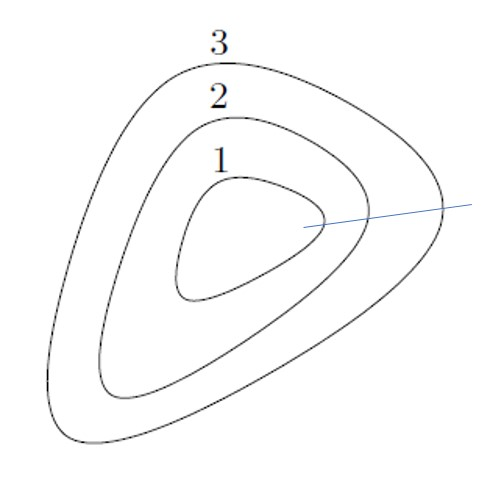
\includegraphics[scale=0.5]{quasiconvex}
	\caption{Quasiconvex}
\end{figure}
